
\documentclass[a4paper,oneside,10pt]{article}
\usepackage[utf8]{inputenc}
\usepackage[T1]{fontenc} 
\usepackage{amsmath,amssymb}
\usepackage{fullpage}
\usepackage{graphicx}
\usepackage{url}
\usepackage{xspace}
\usepackage[french]{babel}
\usepackage{multicol}
\usepackage{geometry}
\usepackage{float}
\geometry{hmargin=2cm,vmargin=1.8cm}
\title{Projet ACVL - Rapport}

\author{DANTIGNY Raynald, DE GEA Jordan, DUCLOT William, RABOURG Simon}

\begin{document}

\maketitle

\tableofcontents


\pagebreak
\section{Analyse}
\subsection{Diagramme de classes d'analyse}
\begin{figure}[H]
\begin{center}
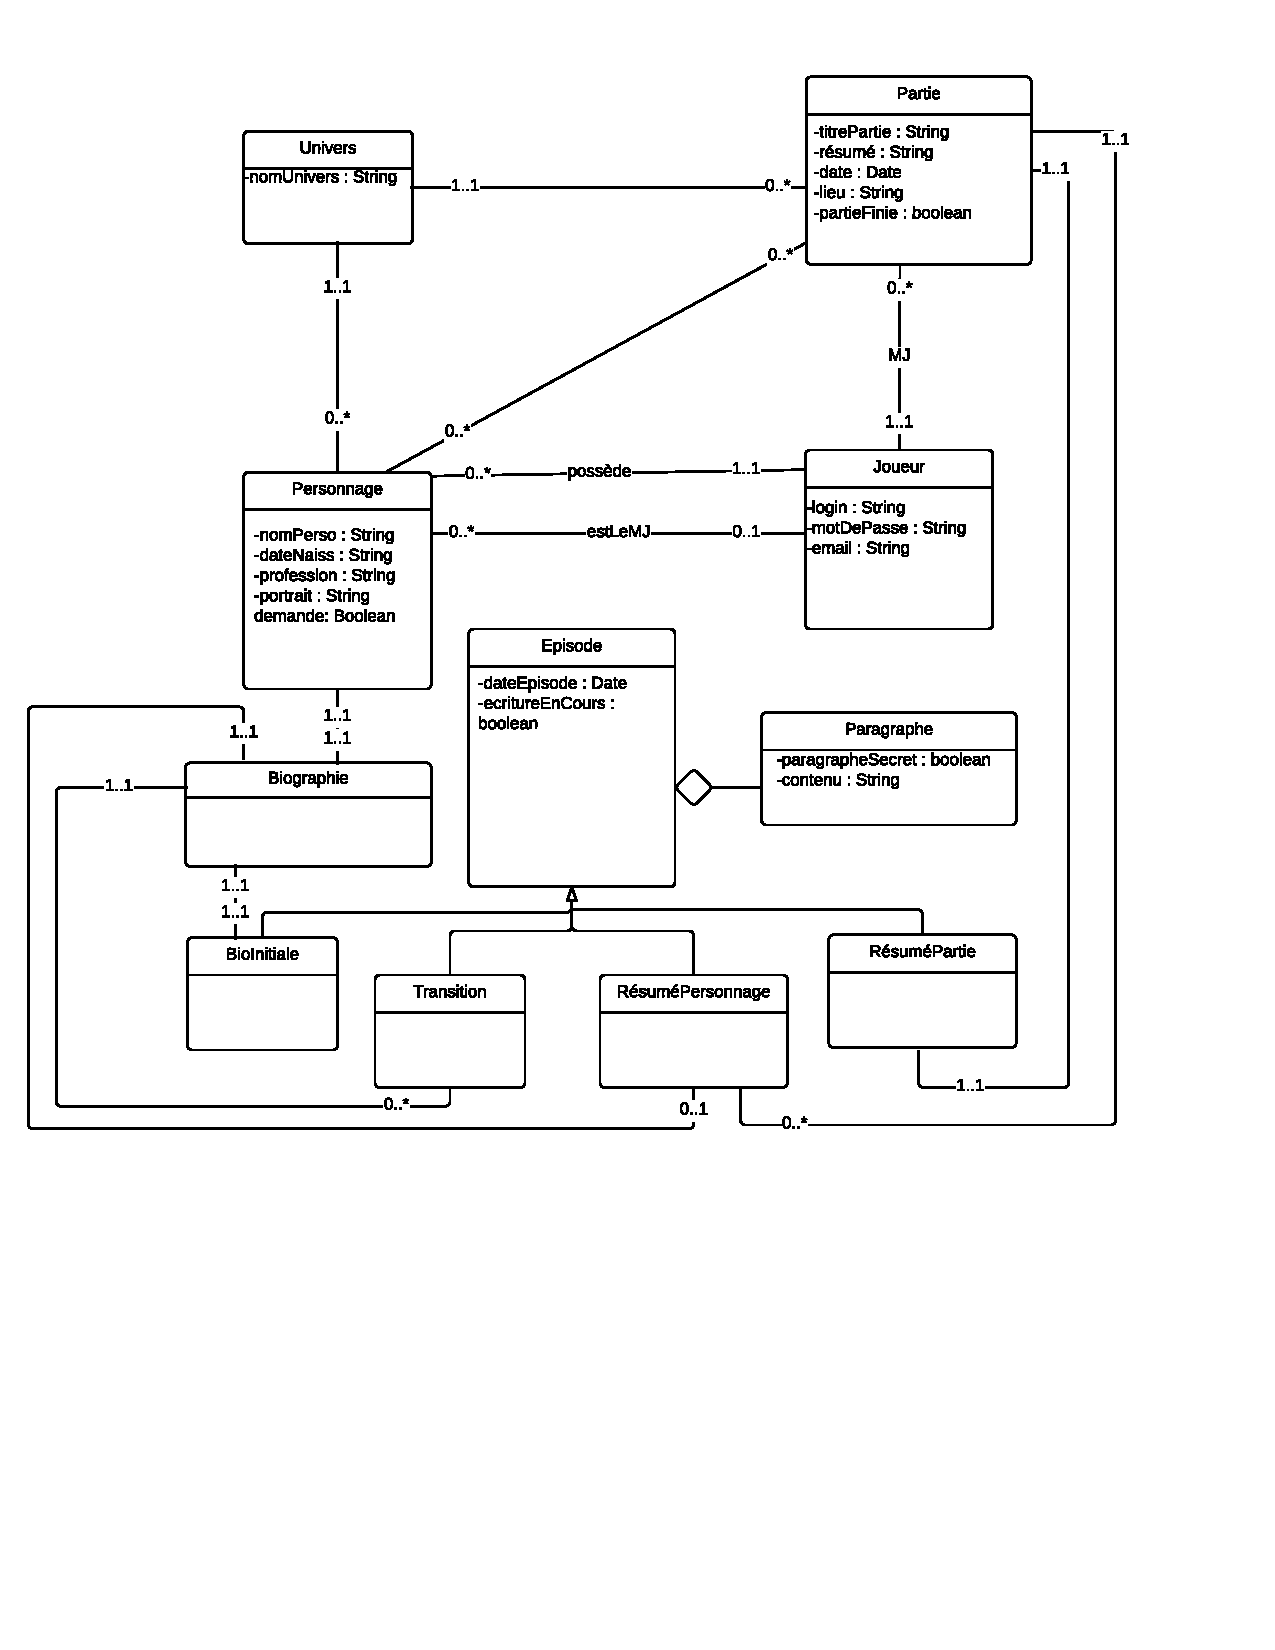
\includegraphics[width=\textwidth]{images/classe/DiagrammeClasse.pdf} 
	\caption{Diagramme de classes d'analyse}
\end{center}
\end{figure}


\pagebreak
\subsection{Cas d'utilisation}

\begin{figure}[H]
	\begin{center}
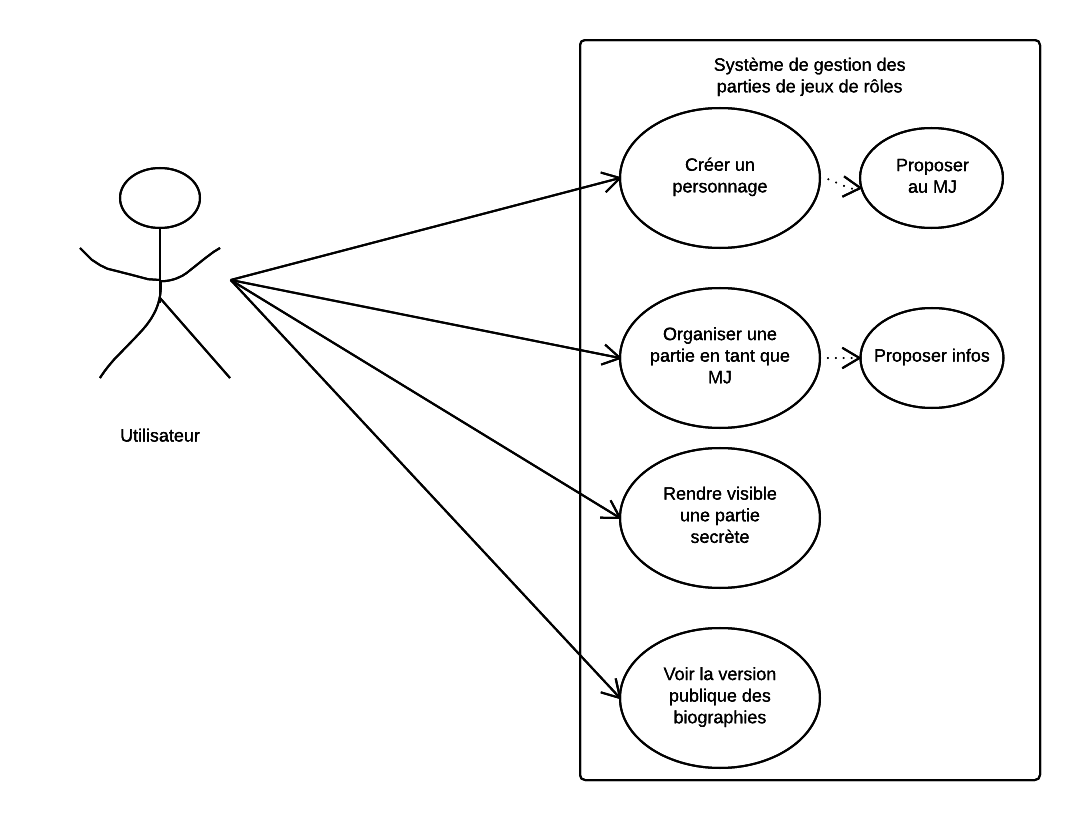
\includegraphics[width=0.6\textwidth]{images/utilisation/UserCU.png} 
	\caption{Cas d'utilisation pour l'utilisateur}
\end{center}
\end{figure}
\begin{figure}[H]
	\begin{center}
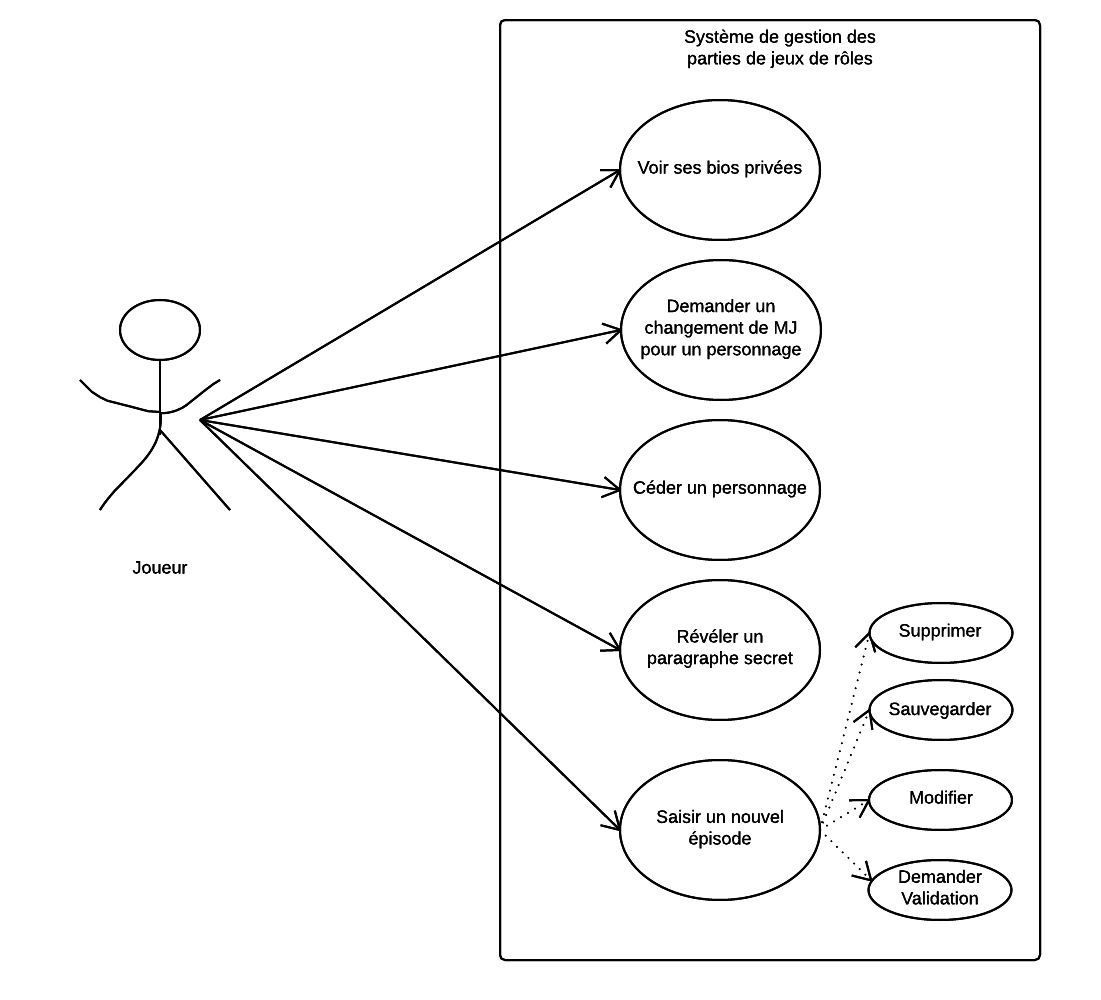
\includegraphics[width=0.49\textwidth]{images/utilisation/JoueurCU.png}
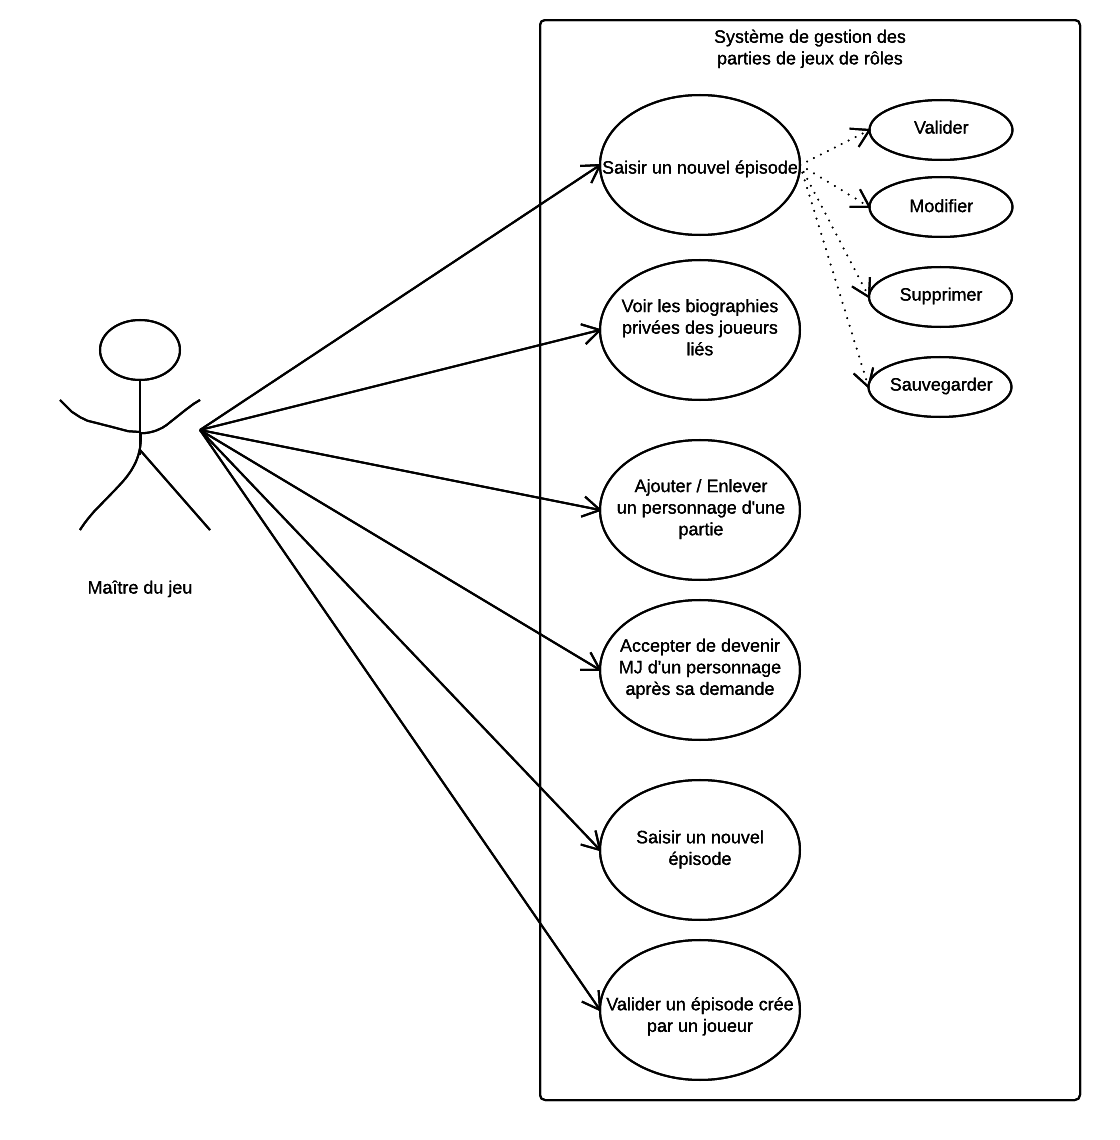
\includegraphics[width=0.49\textwidth]{images/utilisation/MJCU.png}  
	\caption{Cas d'utilisation pour le joueur et le Maitre du Jeu}
\end{center}
\end{figure}

\pagebreak
\subsection{Diagrammes de séquence système}
\begin{figure}[H]
	\begin{center}
		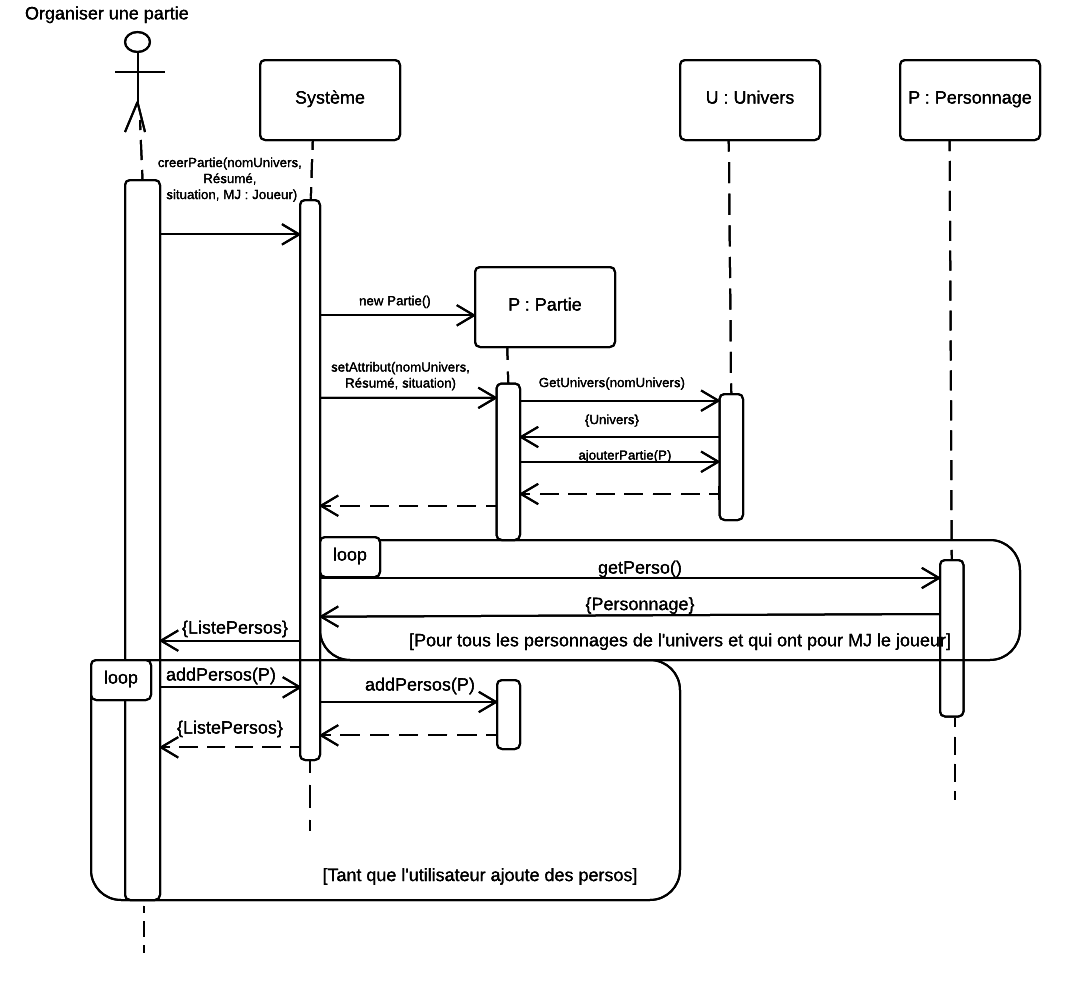
\includegraphics[width=12cm]{images/sequence/DS-OrganiserPartie.png}  
		\caption{Organiser une partie}
	\end{center}
\end{figure}
\begin{figure}[H]
	\begin{center}
		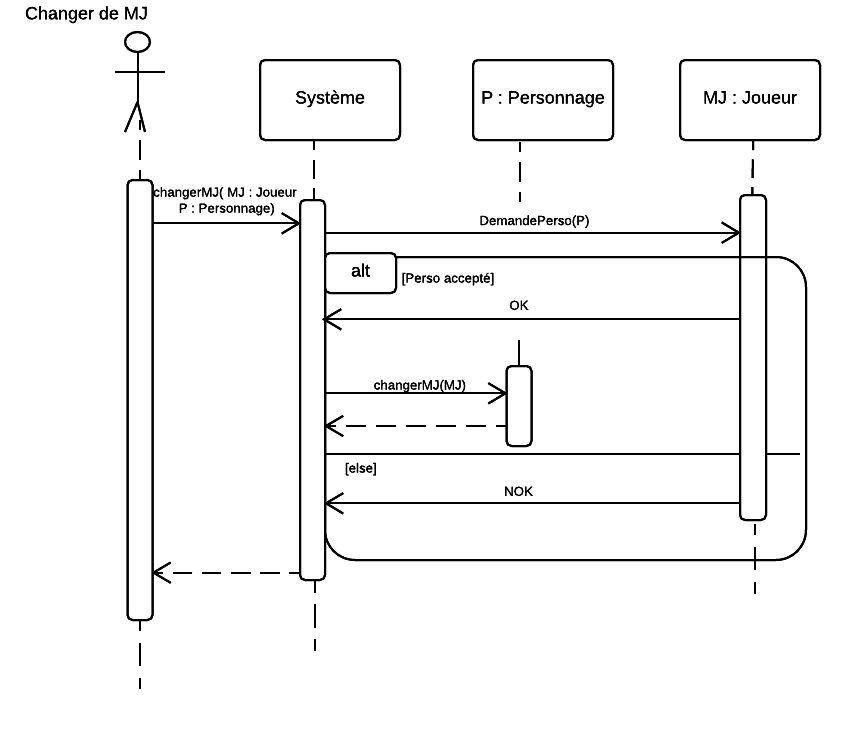
\includegraphics[width=12cm]{images/sequence/DS-ChangerMJ.png}  
		\caption{Changer de maître du jeu pour un personnage}
	\end{center}
\end{figure}
\begin{figure}[H]
	\begin{center}
		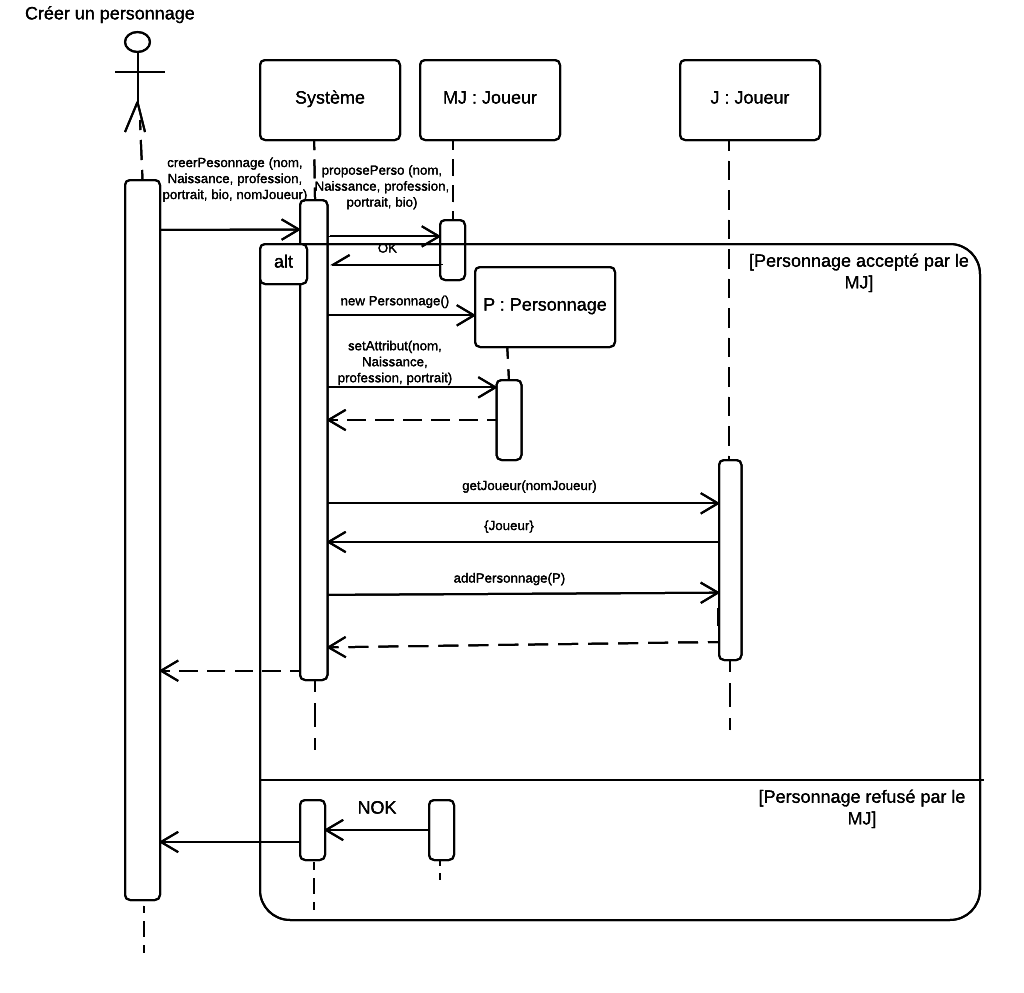
\includegraphics[width=12cm]{images/sequence/DS-CreerPerso.png}  
		\caption{Créer un personnage}
	\end{center}
\end{figure}


\pagebreak

\section{Conception}


\subsection{Diagramme d'architecture MVC}

Voici un exemple pour l'utilisation de l'ensemble \textbf{Partie} :
La vue etant composé de HTML, nous n'avons pas de lien vers des JLabel, JButton, etc. 
Afin d'alleger les heritages, interfaces, etc, nous préferrons ne pas les ajouter à ce diagrammes et vous montrer sur le diagramme de classe logiciel. 

\begin{figure}[H]
	\begin{center}
		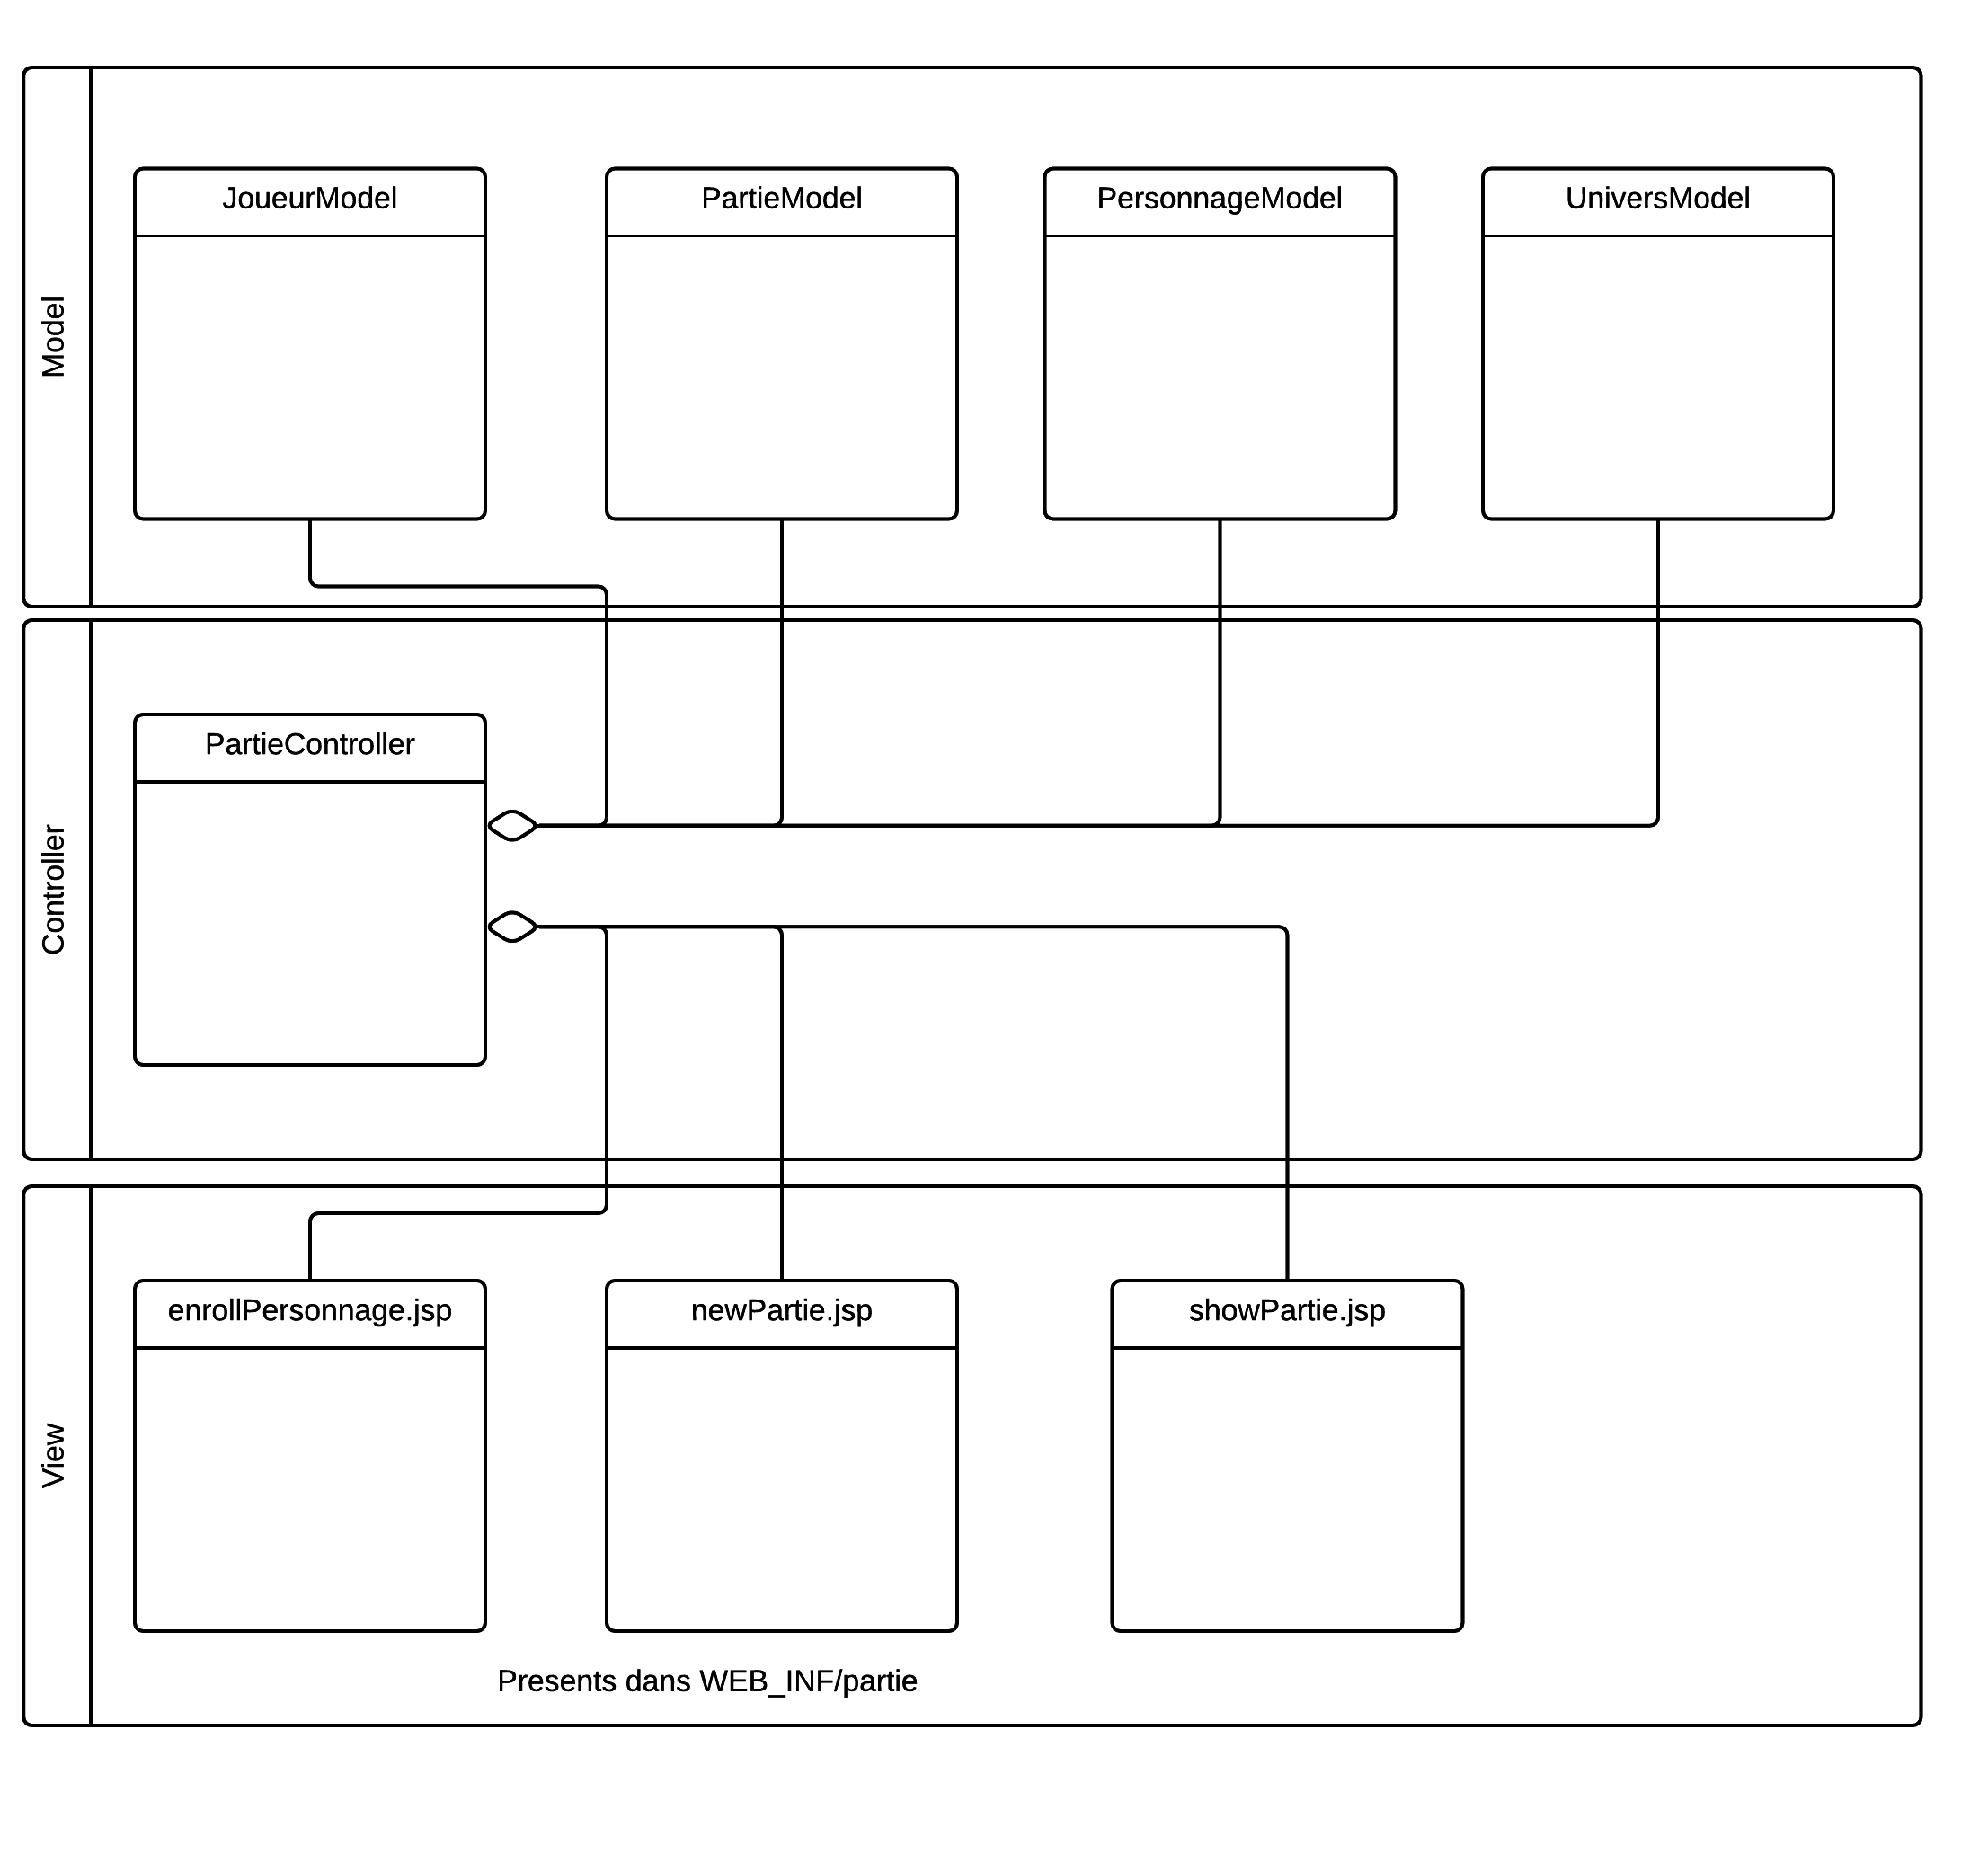
\includegraphics[width=12cm]{images/MVC/model1.png}  
		\caption{MVC pour Partie}
	\end{center}
\end{figure}

\subsection{Diagramme de classe logiciel}

Le nombre de classe étant conséquent, nous préférons vous montrez l'architecture générale de notre application. 


\subsection{Diagramme d'Etats-transitions}
\begin{figure}[H]
	\begin{center}
		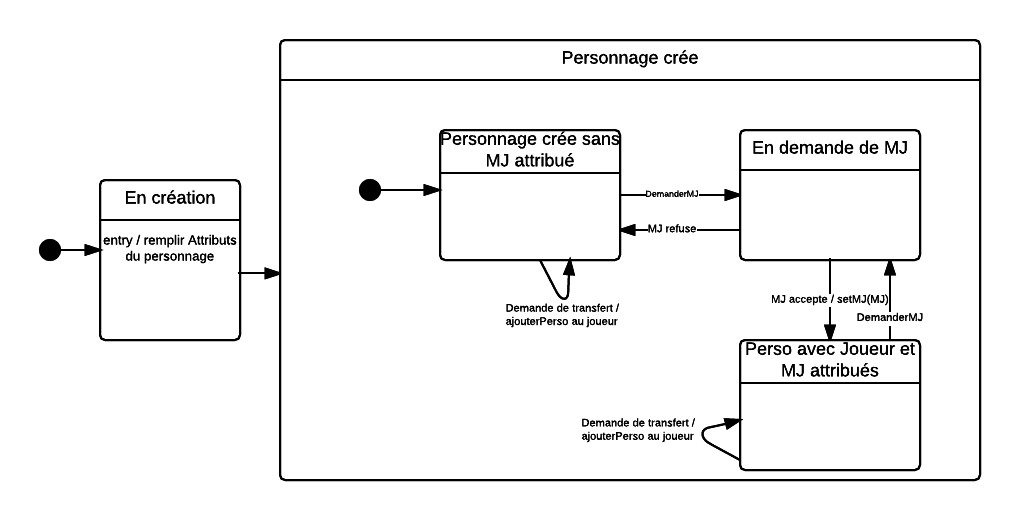
\includegraphics[width=\textwidth]{images/sequence/ET-Personnage.png}  
		\caption{Diagramme d'état/transition pour le changement de MJ et le transfert de personnage}
	\end{center}
\end{figure}

\pagebreak

\section{Manuel Utilisateur}

Chaque page ou fonctionnalité est indiqué en tant que section. 

\subsection{Top Menu}
\label{MUTopMenu}

Le menu affiché en haut de chaque page permet d'accéder rapidement aux différentes fonctions de l'application. Lorsque vous n'êtes pas connecté et quelque soit la page demandé, vous serez redirigé vers la page de Connextion(\ref{MUConnexion}). De cette page, vous pourrez aussi aller à la page d'Inscription(\ref{MUInscription})
Voici les liens menant aux fonctionnalités lorsque vous etes connecté :
\begin{itemize}
	\item Mon profil (\ref{MUProfil})
	\item Parties
	\begin{itemize}
		\item Mes Parties (\ref{MUMesParties})
		\item Voir les parties (\ref{MULesPartiesDisponibles})
	\end{itemize}
	\item Personnages
	\begin{itemize}
		\item Mes Personnages (\ref{MUMesPersonnages})
		\item Voir les personnages (\ref{MULesPersonnagesDisponibles})
	\end{itemize}
	\item Maitre Joueur
	\begin{itemize}
		\item Demandes de joueurs (\ref{MUMJLesDemandes})
		\item Liste de joueurs (\ref{MUMJLesJoueurs})
	\end{itemize}
	\item Episodes 
	\begin{itemize}
		\item Resume
	\end{itemize}
	\item Espace Membre
	\begin{itemize}
		\item Logout : Permet de se déconnecter
	\end{itemize}
\end{itemize}

\subsection{Membre}

\subsubsection{Connexion}
\label{MUConnexion}

Affiche un formulaire de connexion simple. 
\begin{figure}[H]
	\begin{center}
		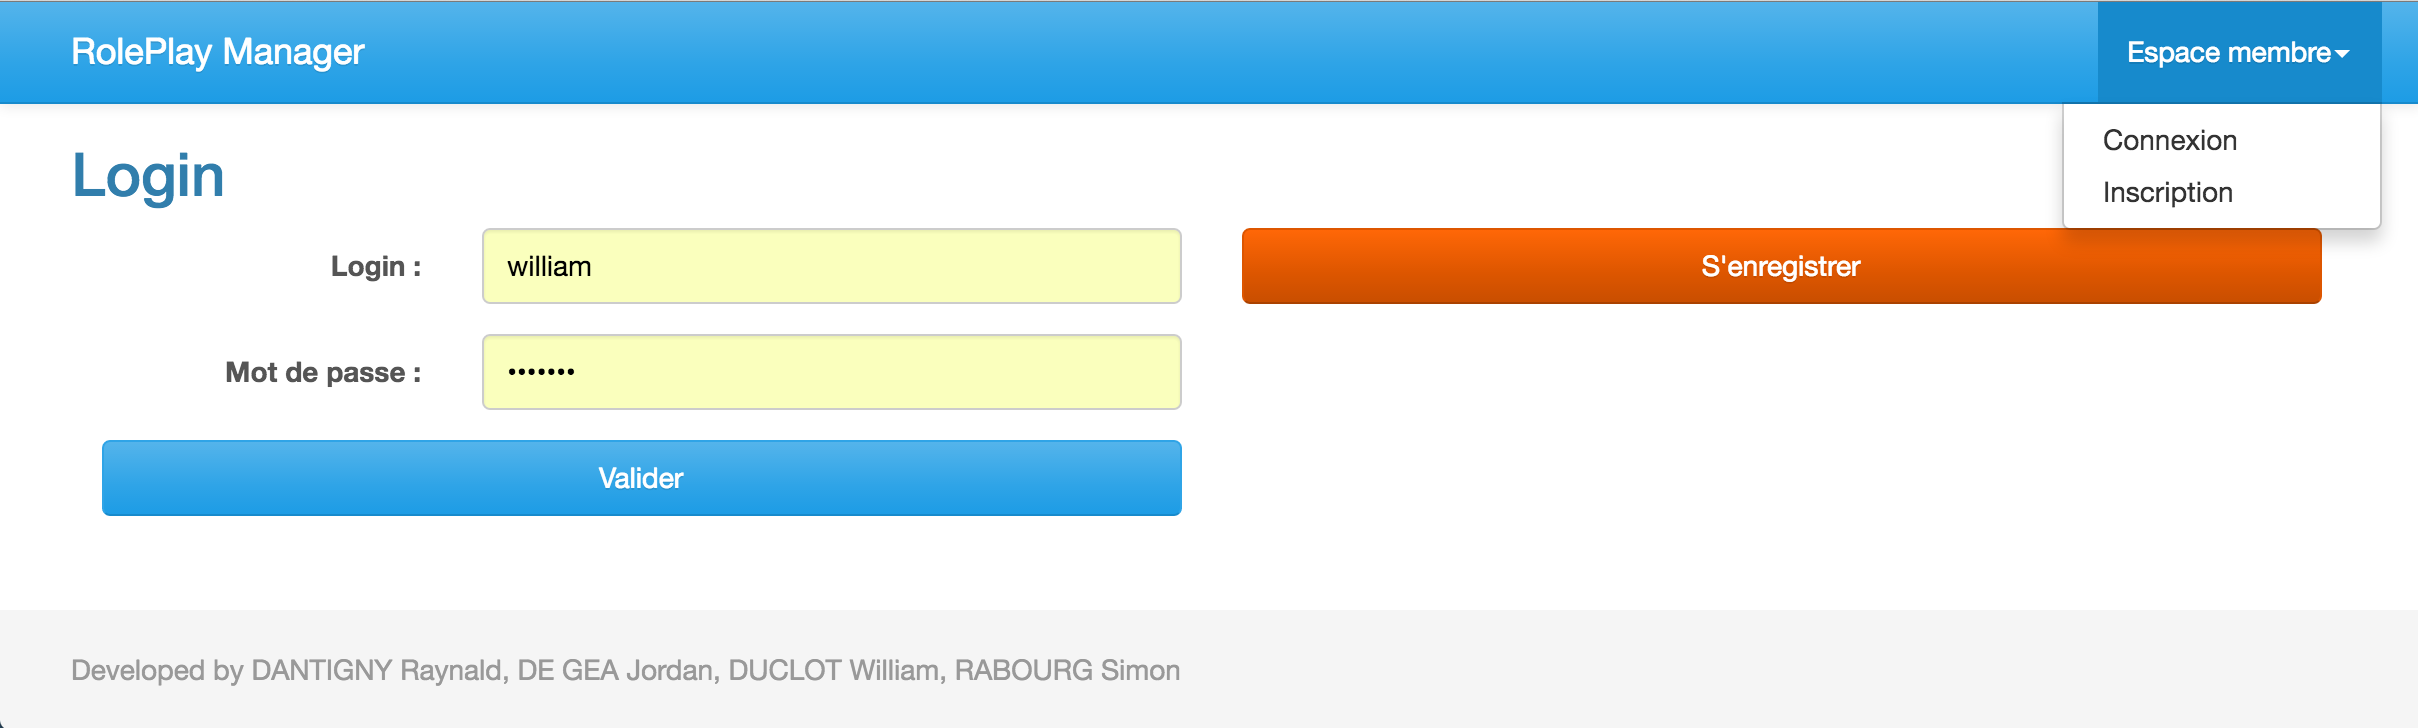
\includegraphics[width=\textwidth]{images/manuel/login.png}  
		\caption{Page de connexion}
	\end{center}
\end{figure}


\subsubsection{Inscription}
\label{MUInscription}

Affiche un formulaire d'inscription avec les champs : login, mot de passe, confirmation et email. 

Si le compte existe déjà, un message d'erreur sera affiché. Sinon, vous êtes redirigé vers la page de profil. 
\begin{figure}[H]
	\begin{center}
		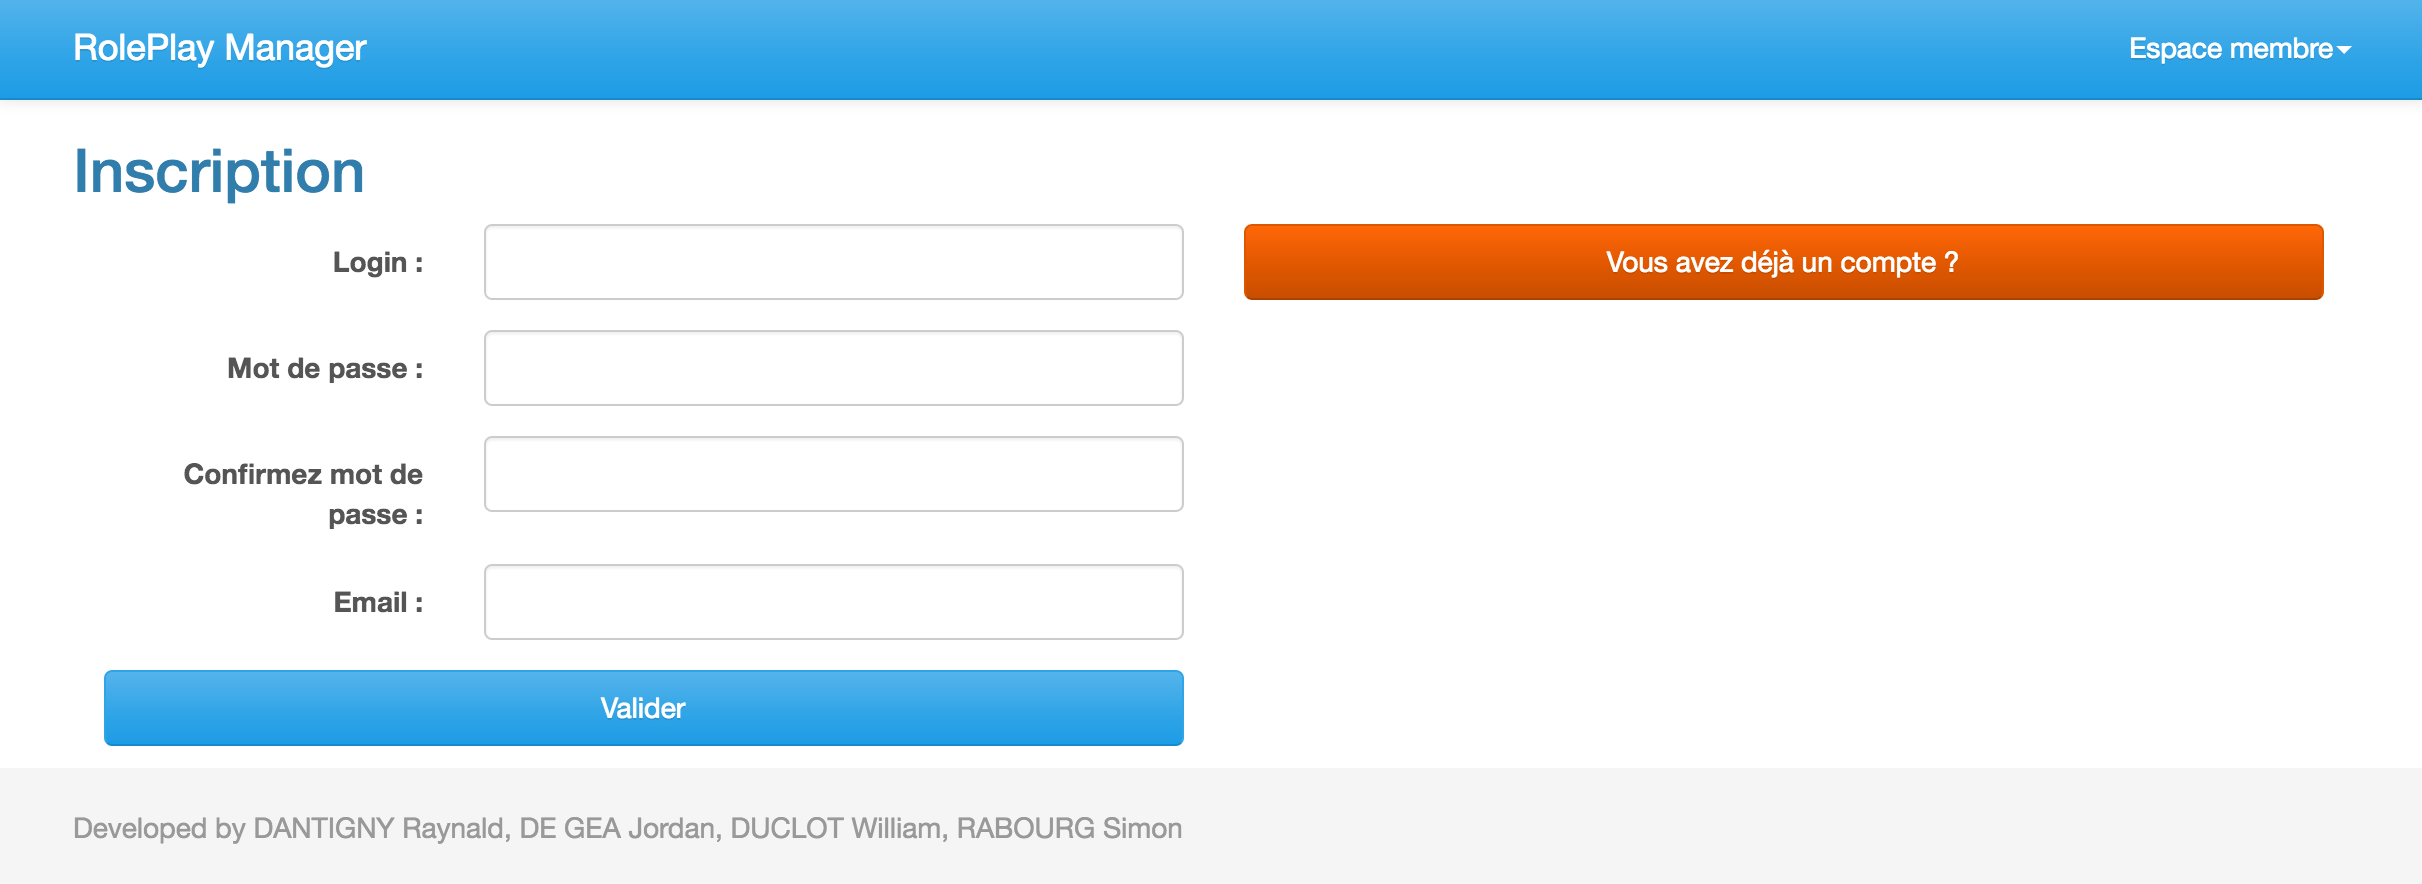
\includegraphics[width=\textwidth]{images/manuel/register.png}  
		\caption{Page d'inscription}
	\end{center}
\end{figure}

\subsubsection{Profil}
\label{MUProfil}

\begin{figure}[H]
	\begin{center}
		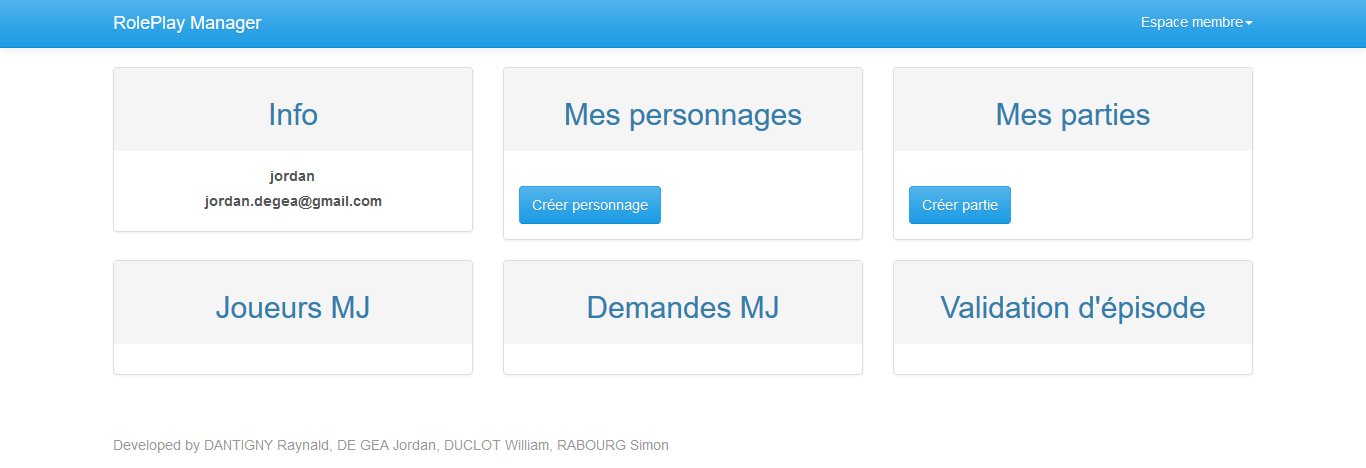
\includegraphics[width=\textwidth]{images/manuel/profil.png}  
		\caption{Page d'accueil de joueur - Profil}
	\end{center}
\end{figure}


\subsection{Parties}

\subsubsection{Créer une Partie}
\label{MUCreerPartie}
\begin{figure}[H]
	\begin{center}
		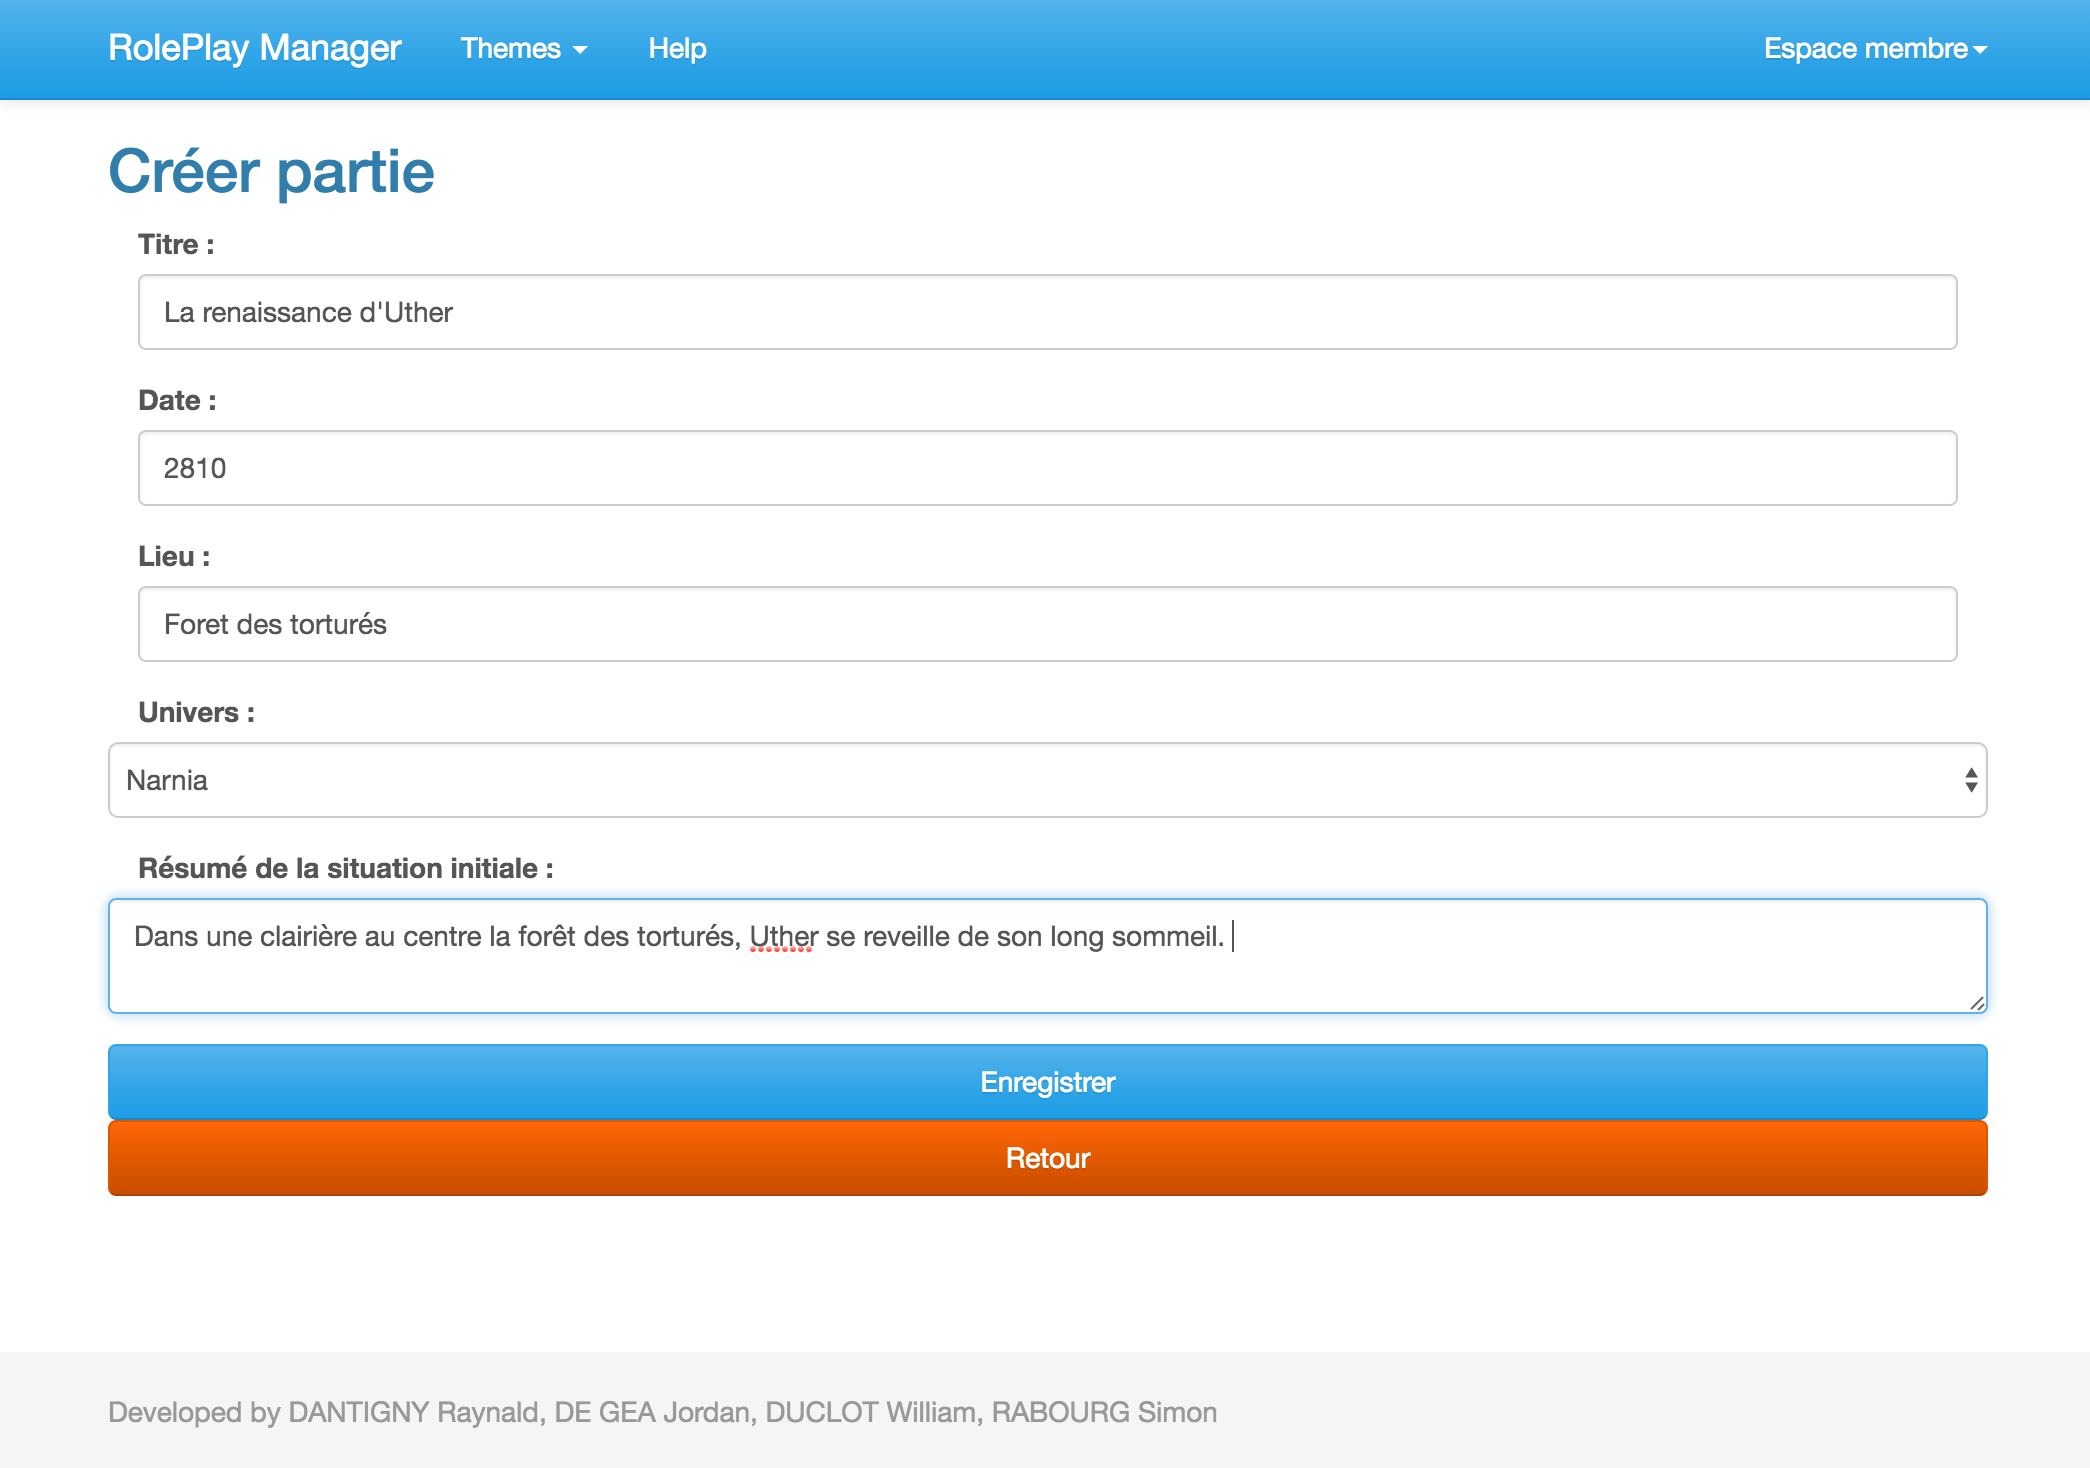
\includegraphics[width=\textwidth]{images/manuel/creerpartie.png}  
		\caption{Page de creation de partie}
	\end{center}
\end{figure}

\subsubsection{Mes Parties}
\label{MUMesParties}

Vous pouvez voir vos parties sur la page de profil

\subsubsection{Les Parties Disponibles}
\label{MULesPartiesDisponibles}

\subsubsection{Voir la Partie}
\label{MUVoirLaPartie}

Lors de l'appui sur un lien \textit{voir} associé à une partie, vous arrivez sur cette page

\begin{figure}[H]
	\begin{center}
		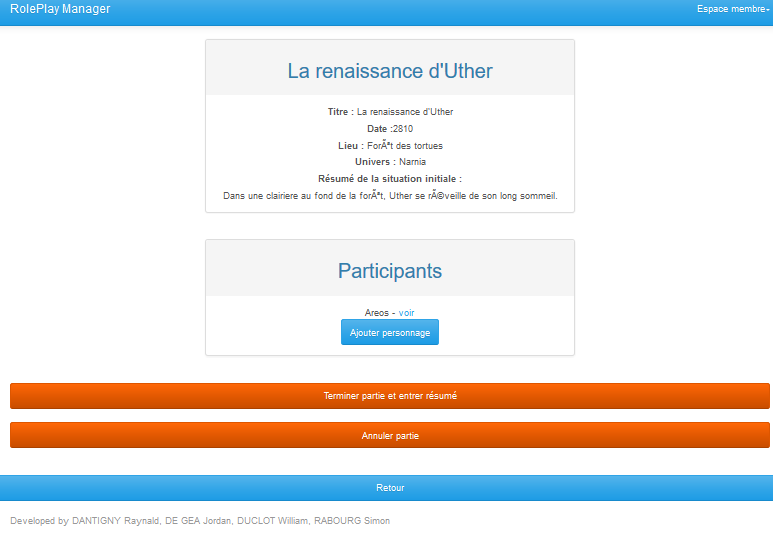
\includegraphics[width=\textwidth]{images/manuel/voirpartie.png}  
		\caption{Page de visualisation de partie}
	\end{center}
\end{figure}

\subsubsection{Ajouter un personnage à la partie}
\label{MUAjouterPersonnagePartie}


\begin{figure}[H]
	\begin{center}
		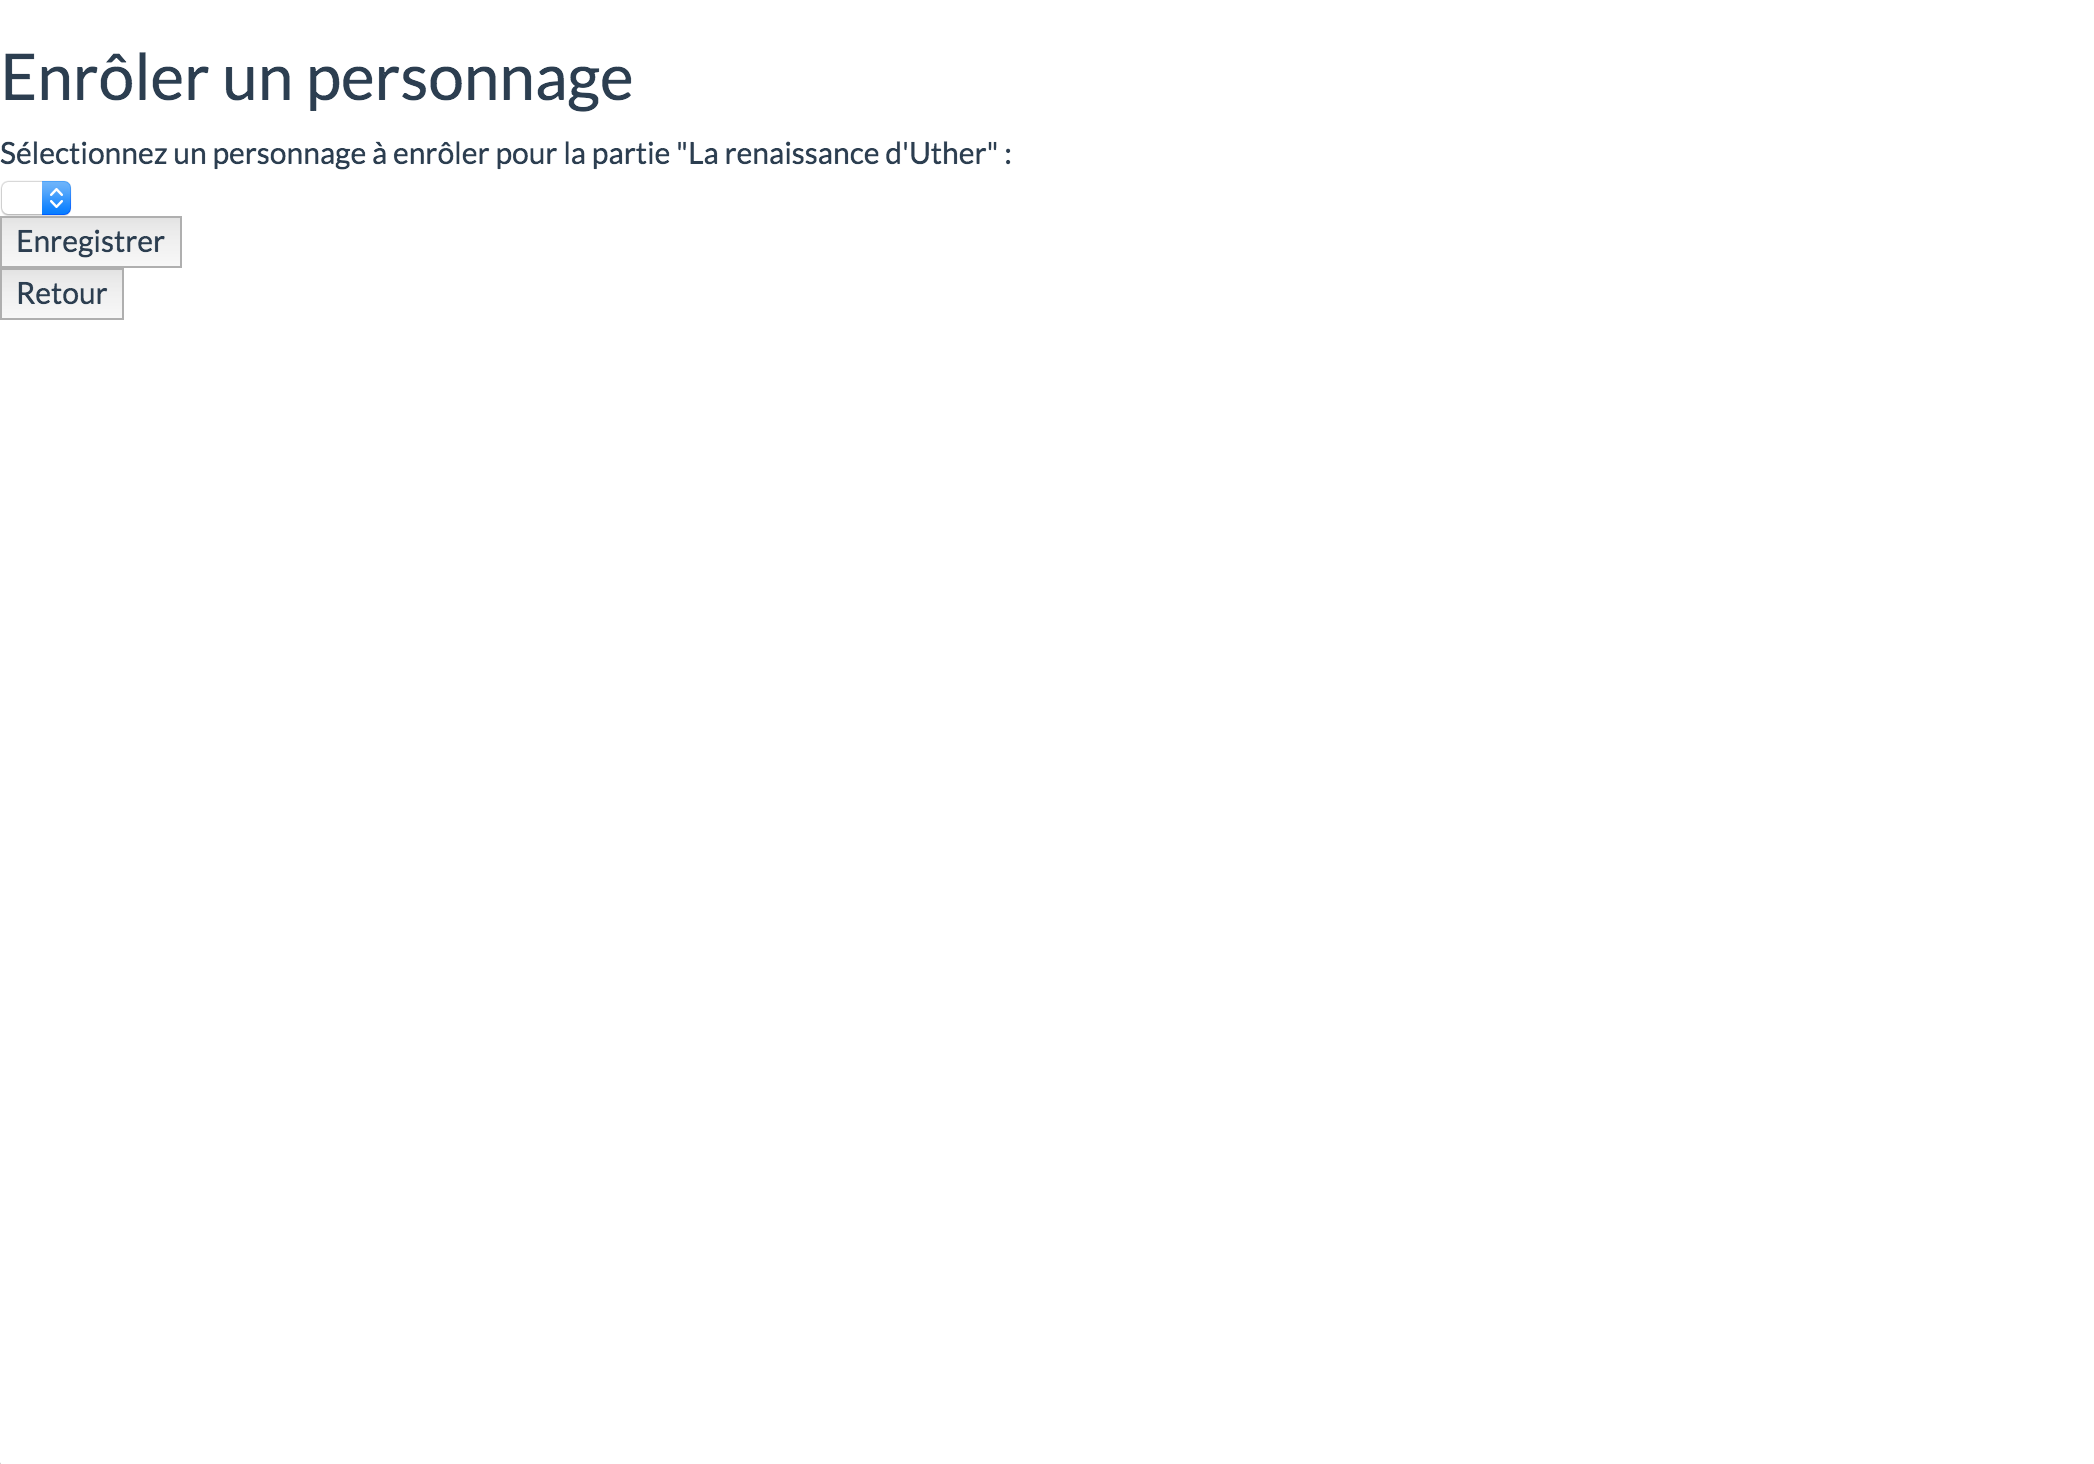
\includegraphics[width=10cm]{images/manuel/enroll.png}  
		\caption{Page d'ajout de personnage à une partie}
	\end{center}
\end{figure}

\subsection{Personnages}

\subsubsection{Créer un Personnage}
\label{MUCreerPersonnage}

\begin{figure}[H]
	\begin{center}
		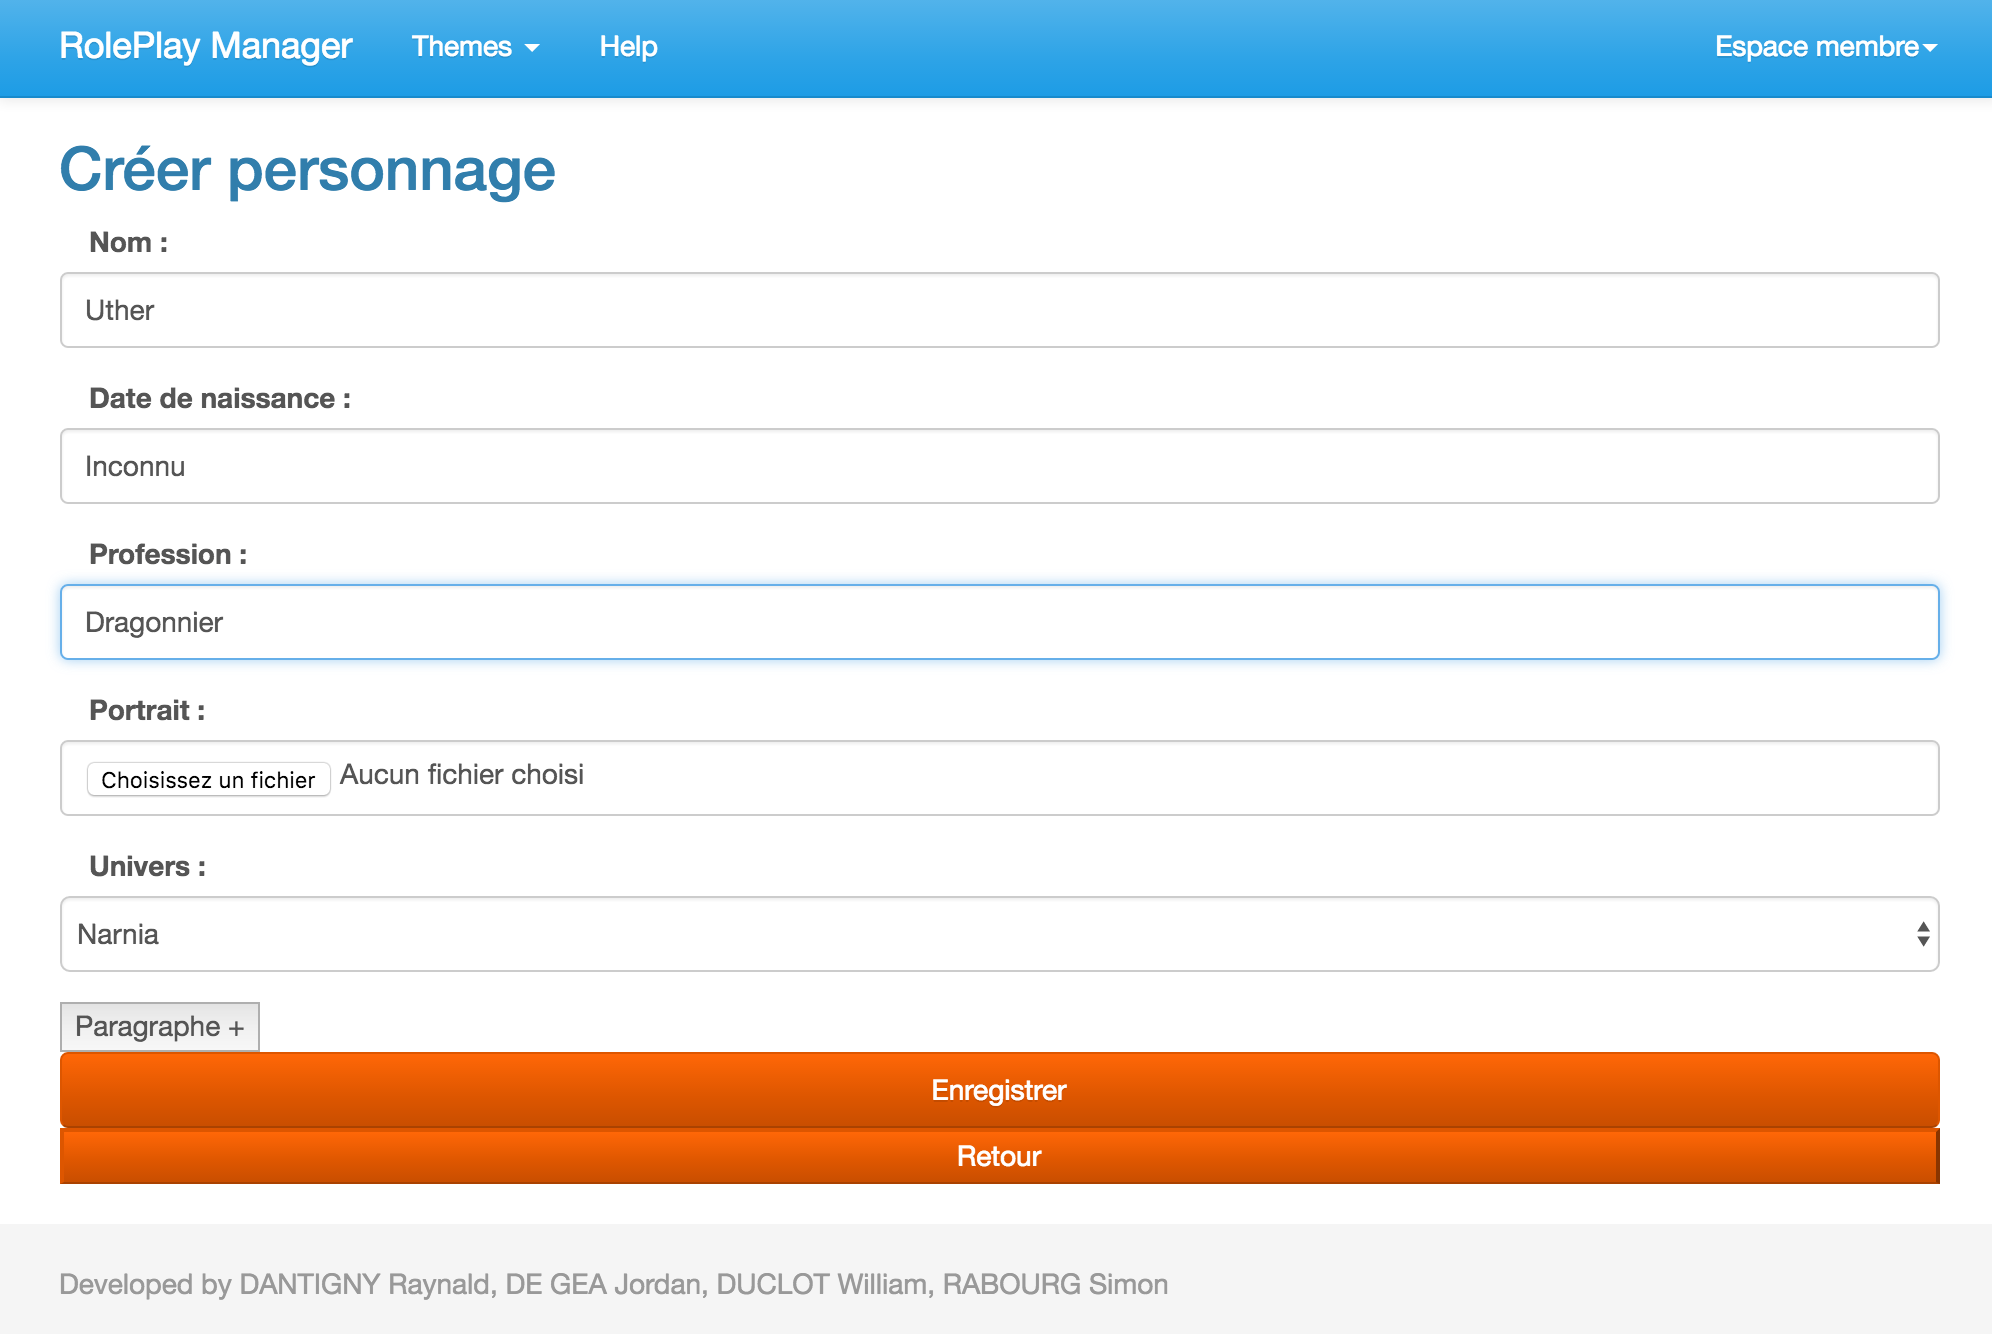
\includegraphics[width=\textwidth]{images/manuel/creerpersonnage.png}  
		\caption{Page de creation de personnage}
	\end{center}
\end{figure}

\subsubsection{Modifier un Personnage}
\label{MUModifierPersonnage}

\begin{figure}[H]
	\begin{center}
		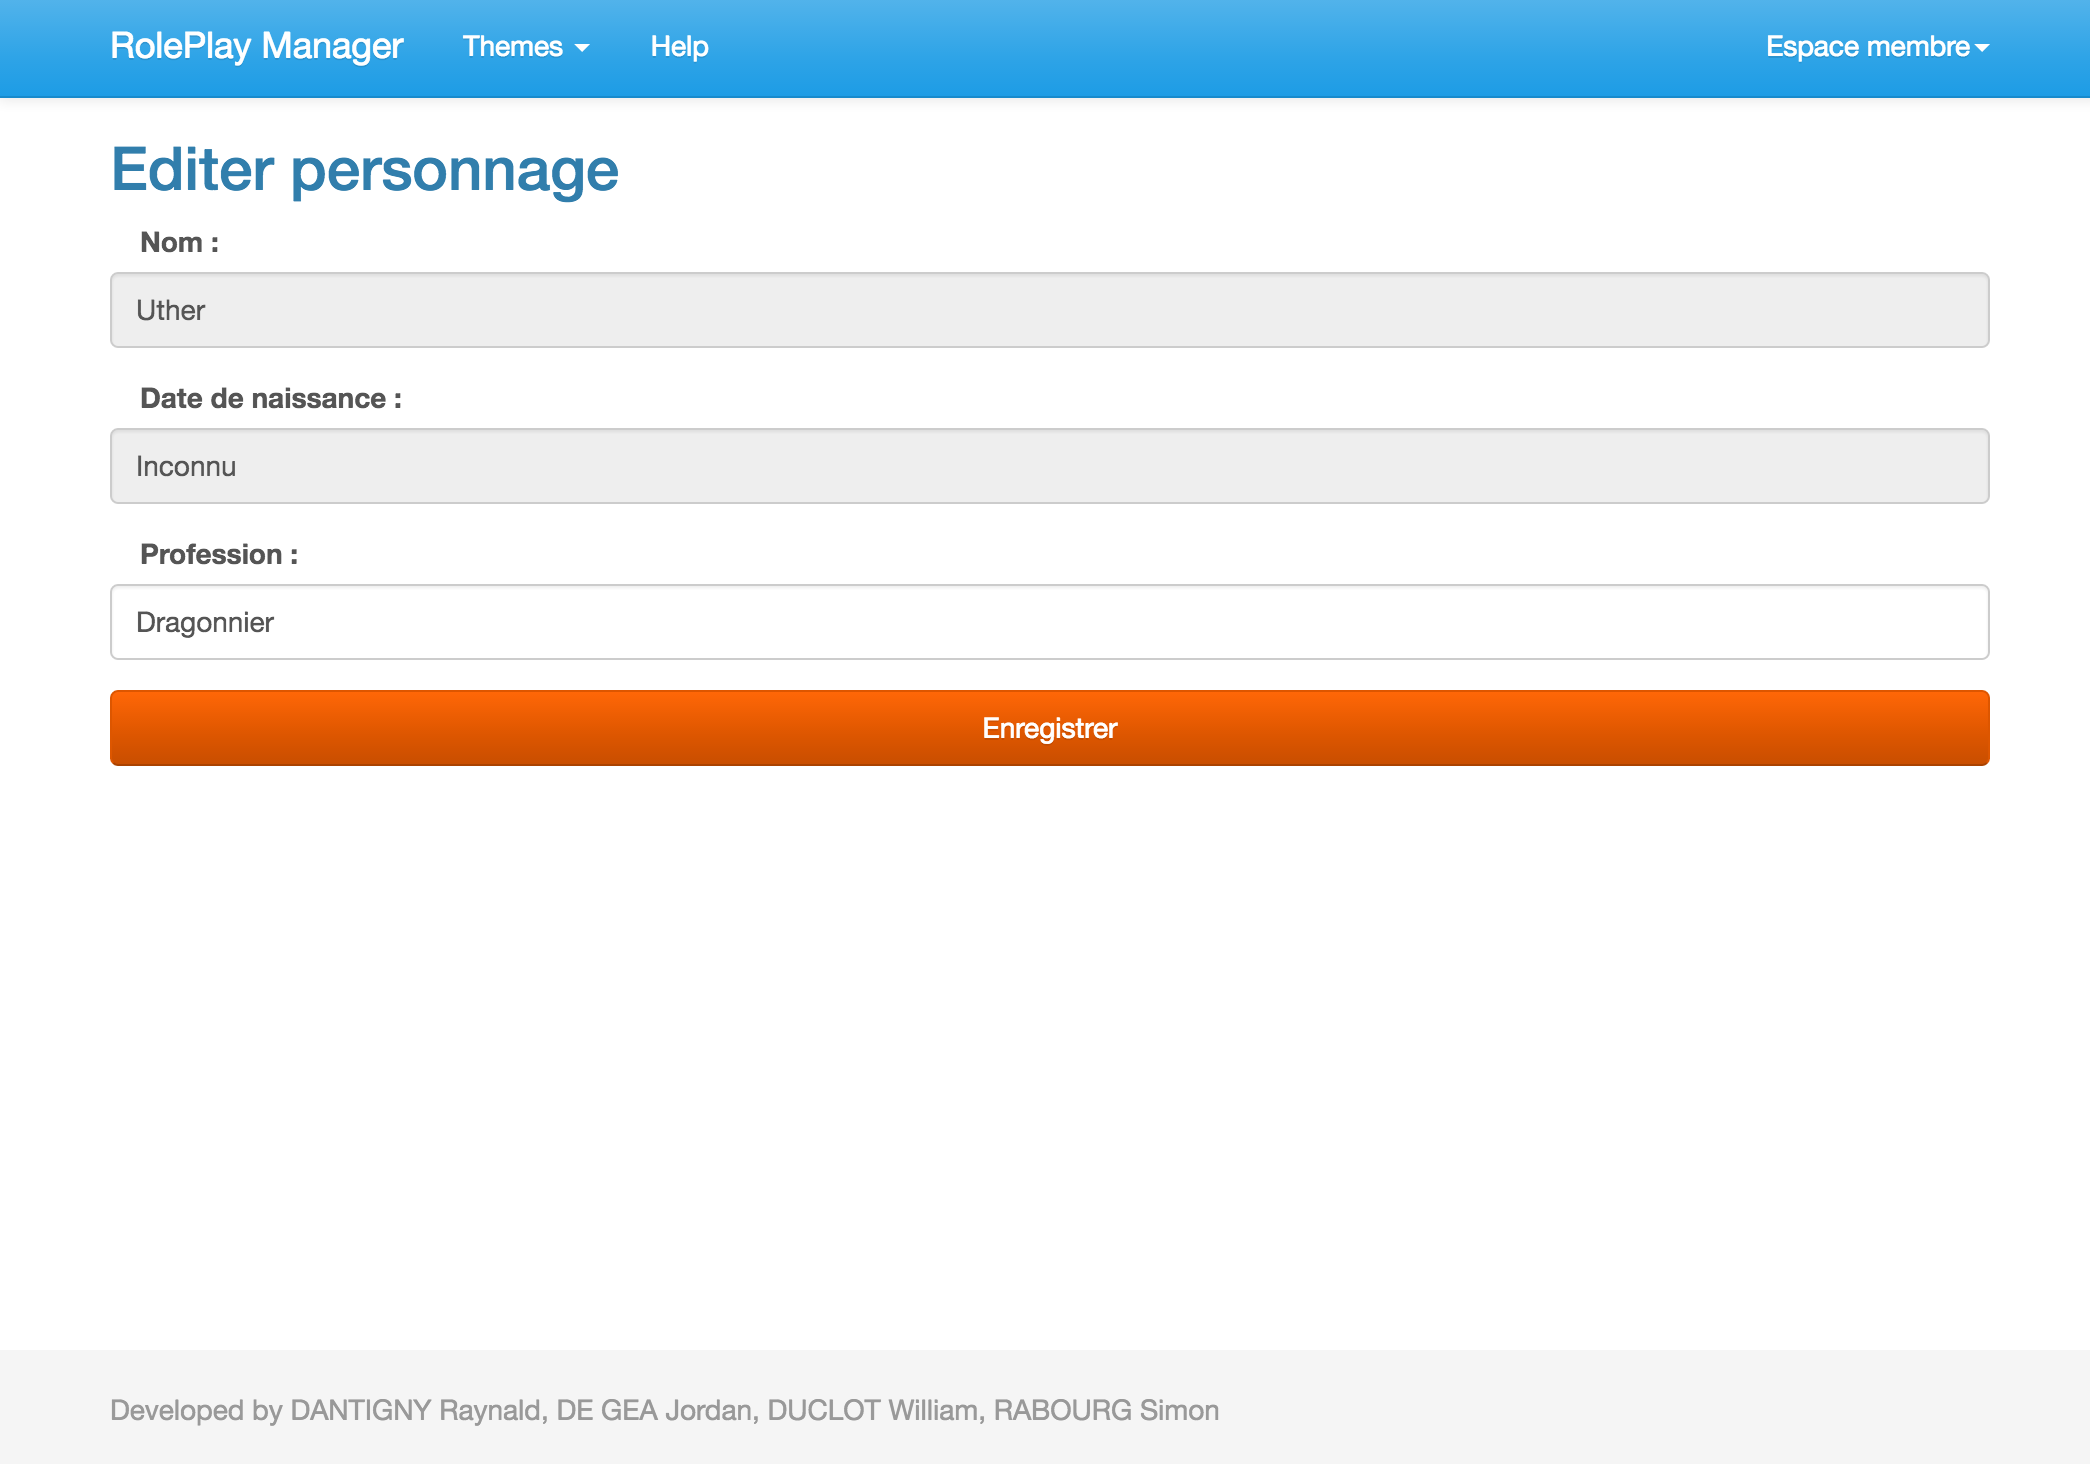
\includegraphics[width=\textwidth]{images/manuel/editerpersonnage.png}  
		\caption{Page d'edition de personnage}
	\end{center}
\end{figure}

\subsubsection{Mes Personnages}
\label{MUMesPersonnages}

Vous pouvez voir la liste des personnages sur votre page de profil. 

\subsubsection{Les Personnages Disponibles}
\label{MULesPersonnagesDisponibles}


\subsubsection{Voir le Personnage}
\label{MUVoirLePersonnage}

\begin{figure}[H]
	\begin{center}
		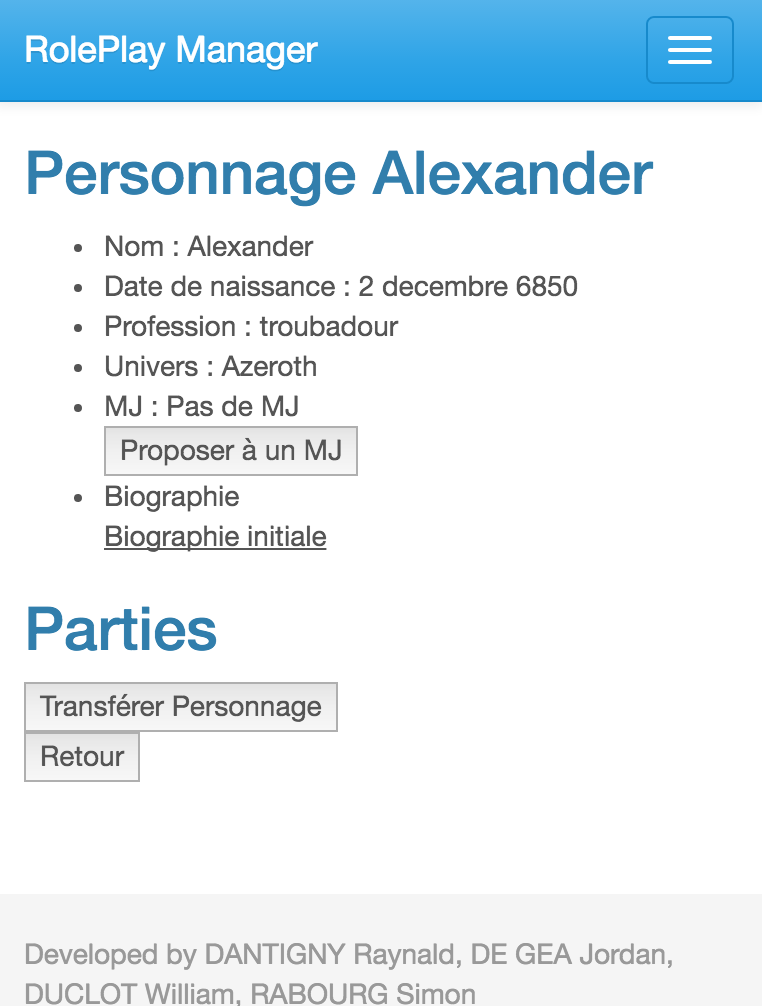
\includegraphics[width=5cm]{images/manuel/voirpersonnage.png}  
		\caption{Page de visualisation de personnage}
	\end{center}
\end{figure}

\subsubsection{Ajouter un MJ au personnage}
\label{MUAjouterMJPersonnage}


Sur la page "Voir le Personnage", vous avez un bouton Proposer à un MJ. Ce bouton vous redirige sur cette page. 

\begin{figure}[H]
	\begin{center}
		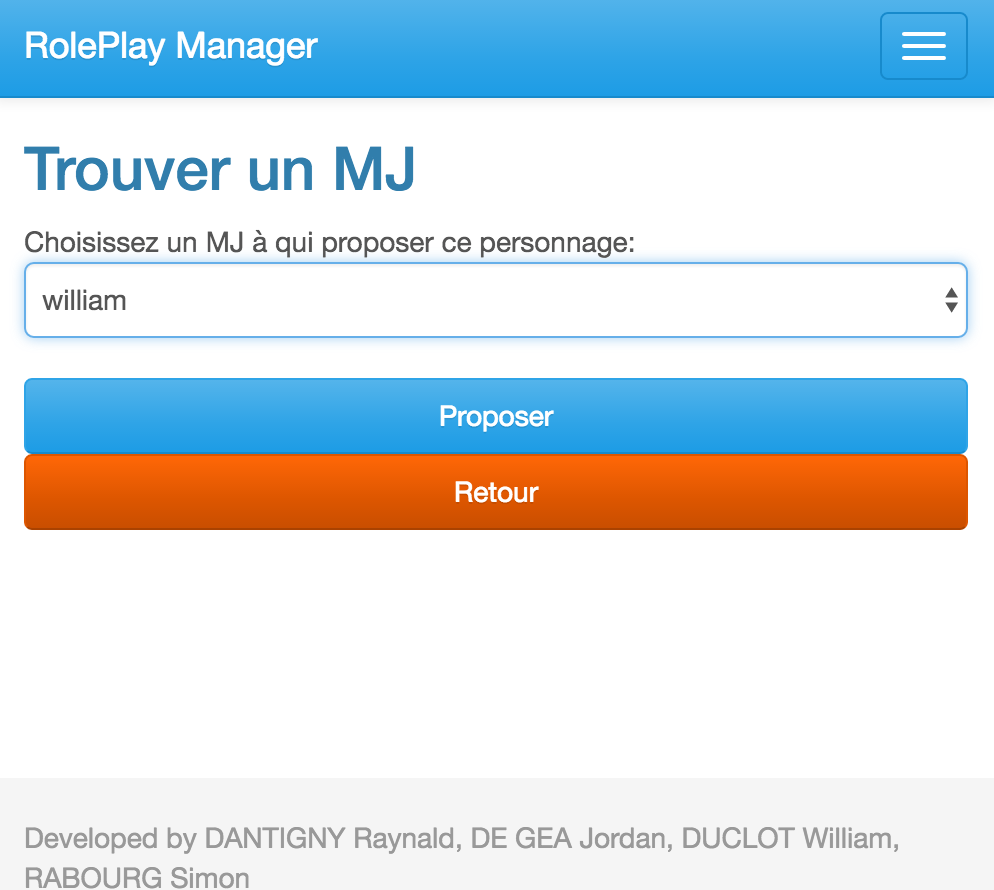
\includegraphics[width=5cm]{images/manuel/trouverMJ.png}  
		\caption{Page pour cherche un MJ}
	\end{center}
\end{figure}

Une fois la demande effectué, voici l'état de la page "Voir Le Personnage". En cliquant sur "Quitter ce MJ", vous revenez à l'état de la page dans la section "Voir Le Personnage". 

\begin{figure}[H]
	\begin{center}
		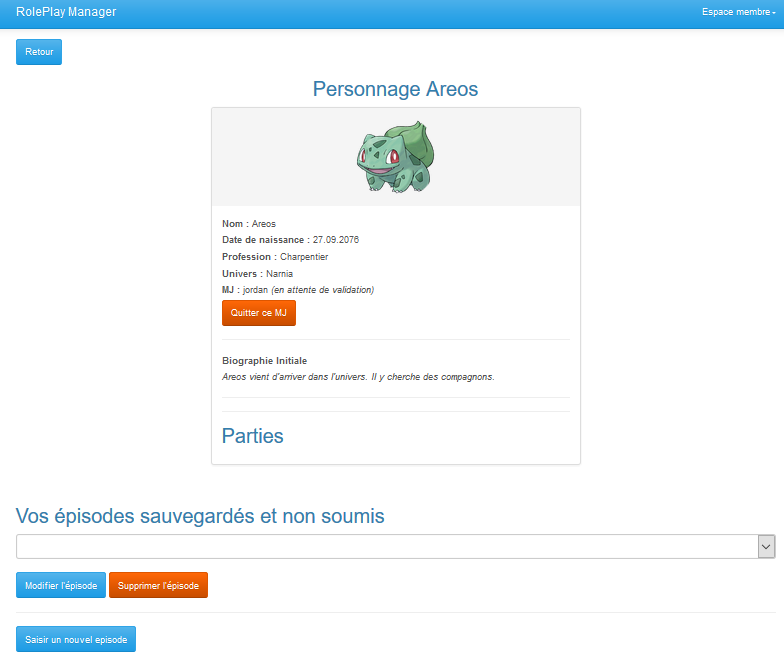
\includegraphics[width=5cm]{images/manuel/voirpersonnagedemandeMJ.png}  
		\caption{Page de personnage apres la recherche}
	\end{center}
\end{figure}


\subsection{MJ}

\subsubsection{MJ : Les Demandes}
\label{MUMJLesDemandes}

La page profil ressemble à cette image lorsqu'une personne vous demande comme MJ. Vous pouvez Accepter ou Refuser. En Acceptant, ce personnage est ajouté à la catégorie "Joueur MJ"
\begin{figure}[H]
	\begin{center}
		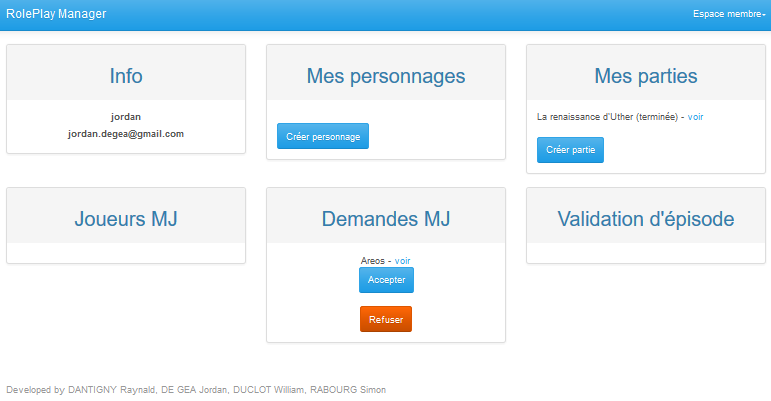
\includegraphics[width=\textwidth]{images/manuel/profildemande.png}  
		\caption{Page pour cherche un MJ}
	\end{center}
\end{figure}



\subsubsection{MJ : Les Joueurs}
\label{MUMJLesJoueurs}

La page de profil vous montre tous les joueurs vous ayant comme MJ.


\pagebreak

\section{Bilan}

%Bilan sur les outils de modélisation utilisés, en particulier les problèmes rencontrés, ainsi que les solutions trouvées. Il vous est demandé dans cette partie de bien préciser les logiciels, en particulier les modeleurs UML que vous avez utilisés.

\subsection{Recherche de modeleurs UML}

Nous avons fait une courte recherche de modeleurs, mais aucun de ceux proposés spécialement en tant que Modeleur ne nous convenait. Nous nous sommes donc dirigé vers un outil que nous connaissons : LucidChart. LucidChart est un outil connecté à GoogleDrive permettant de faire des schémas, d'UML entre autre. 


\subsection{Outil : LucidChart}

Nous avons utilisé LucidChart pour : 
\begin{itemize}
	\item Diagramme de classe d'analyse
	\item Diagramme de séquence système
	\item Cas d'utilisation
\end{itemize}

Difficultés : C'est pratique car c'est personnalisable mais pas forcement adapté pour l'UML. L'utilisation n'est pas simple et intuitive. 

\subsection{IDE : Netbeans}

Nous avons tous utilisé Netbeans pour le développement. L'avantage d'avoir le même IDE est qu'il est plus facile d'aider un collègue lors d'un problème. Etant habitué à cet IDE, nous pouvions développer rapidement. 

\subsection{Tomcat8 / JDBC}

Pour le serveur web, nous avons utilisé Tomcat8 . 
JDBC est la library devant être utilisé pour le projet afin de se connecter à la base Oracle.  

\subsection{Latex : TexMaker}

TexMaker est, selon nous, le meilleur éditeur graphique de contenu \LaTeX. 

\subsection{Versionning : GIT}

Le système de version "de base" pour les projets. Hebergé sur Gitlab.com. 




















\end{document}
